\section{Symulacja i weryfikacja}
\label{sec:sym-wer}

Aby sprawdzić poprawność działania algorytmu optymalizacji dynamicznej, wykonano symulacje weryfikacyjne przy użyciu oprogramowania JModelica.org na wyższym poziomie aplikacji oraz środowiska MATLAB/Simulink na niższym.
W obu tych przypadkach błąd weryfikacji jest liczony według wzoru \ref{eq:ver-error}, gdzie $\hat{h_{i}}(T)$ to ostatnia wartość trajektorii odpowiedniego poziomu (po upływie wyliczonego czasu), a $h_{i}^{f}$ to wartość docelowa tego poziomu.

\begin{equation}\label{eq:ver-error}
e_{wer} = \sum_{i=1}^{3} (\hat{h_{i}}(T) - h_{i}^{f})^{2}
\end{equation}

Należy zwrócić uwagę na to, iż weryfikacja poprawności rozwiązania korzysta z innych danych, niż sprawdzenie dokładności rozwiązania opisane w sekcji \ref{sub:opt-dokladnosc}. Pierwsza procedura używa danych symulacyjnych uzyskanych po optymalizacji, a druga - danych pochodzących bezpośrednio z algorytmu optymalizacyjnego.

%-------------------------------------------------
\subsection{Przy użyciu pakietu JModelica.org}
\label{sub:sym-wer-jmodelica}

Po zakończeniu optymalizacji wyższy poziom aplikacji umożliwia przeprowadzenie symulacji weryfikacyjnej. Podaje się wtedy cały uzyskany wektor sterowania optymalnego (w postaci ,,surowej'' lub znormalizowanej) jako trajektorię wejściową do symulacji, a na koniec wylicza się błąd weryfikacji.

Poniżej przedstawiono 2 przykłady wykresów uzyskanych w czasie weryfikacji i porównano wartości błędów przy zastosowaniu sterowania w postaci ,,surowej'' oraz znormalizowanej.

\begin{figure}[htp]
    \centering
    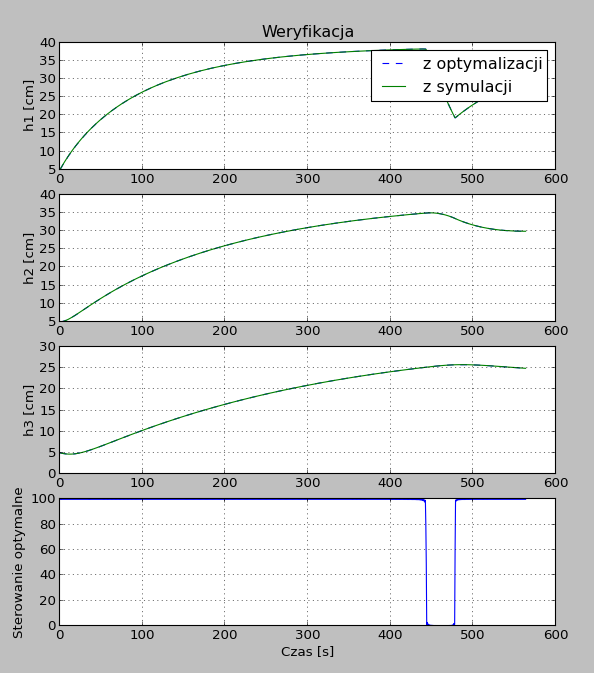
\includegraphics{Grafika/plot_5_5_6-30_30_25-raw-350}
    \caption{Przykładowa weryfikacja rozwiązania przy użyciu pakietu JModelica.org. Źródło: własne.}
    \label{fig:plot556-303035-raw-350}
\end{figure}

\begin{figure}[htp]
    \centering
    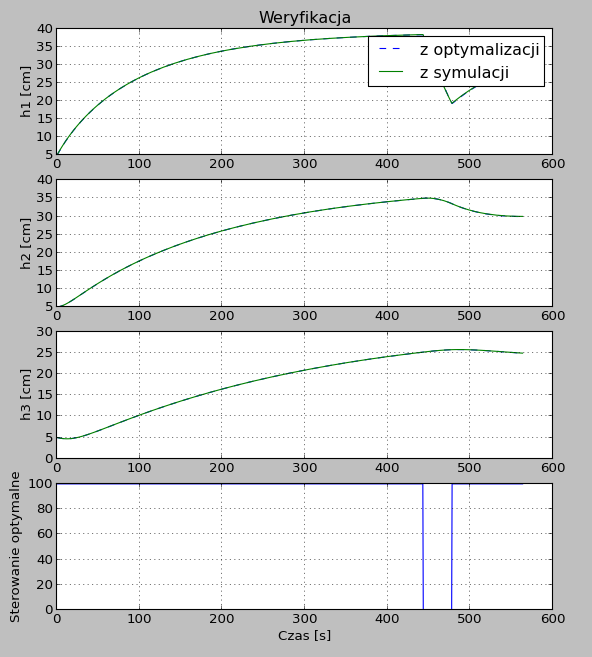
\includegraphics{Grafika/plot_5_5_6-30_30_25-normalised-350}
    \caption{Przykładowa weryfikacja po normalizacji sterowania. Źródło: własne.}
    \label{fig:plot556-303035-normalised-350}
\end{figure}

Pierwszy przykład to napełnianie zbiorników od poziomów $h_{1}^{0} = 5 cm, h_{2}^{0} = 5 cm, h_{3}^{0} = 6 cm$ do poziomów $h_{1}^{f} = 30 cm, h_{2}^{f} = 30 cm, h_{3}^{f} = 25 cm$. Sterowanie w postaci z algorytmu optymalizacji osiągnęło wartość błędu weryfikacji $e_{wer}^{s} = 0,0002$, a po znormalizowaniu: $e_{wer}^{n} = 0.002$. W tym przypadku sterowanie w postaci ,,surowej'' (przedstawione na rys. \ref{fig:plot556-303035-raw-350}) wizualnie nie różni się bardzo od sterowania znormalizowanego (pokazanego na rys. \ref{fig:plot556-303035-normalised-350}), ale nawet taka niewielka różnica może prowadzić do zwiększenia się błędu weryfikacji o rząd wielkości. Jest to jednak również związane z tym, iż pierwszy błąd jest bardzo niewielki i w czasie wielu prób rzadko uzyskiwano tak niewielkie wartości. W tej optymalizacji użyto 350 elementów skończonych.

\begin{figure}[htp]
    \centering
    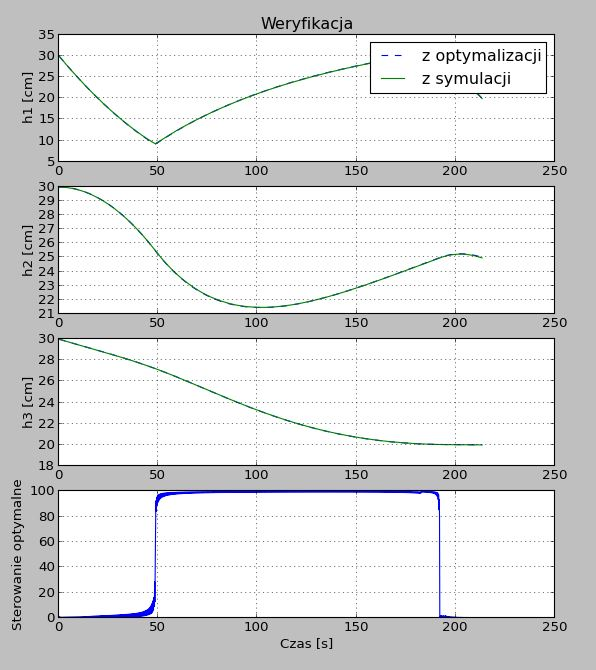
\includegraphics{Grafika/plot_30_30_30-20_25_20_raw_200}
    \caption{Druga przykładowa weryfikacja rozwiązania przy użyciu pakietu JModelica.org. Źródło: własne.}
    \label{fig:plot303030-202520raw200}
\end{figure}

\begin{figure}[htp]
    \centering
    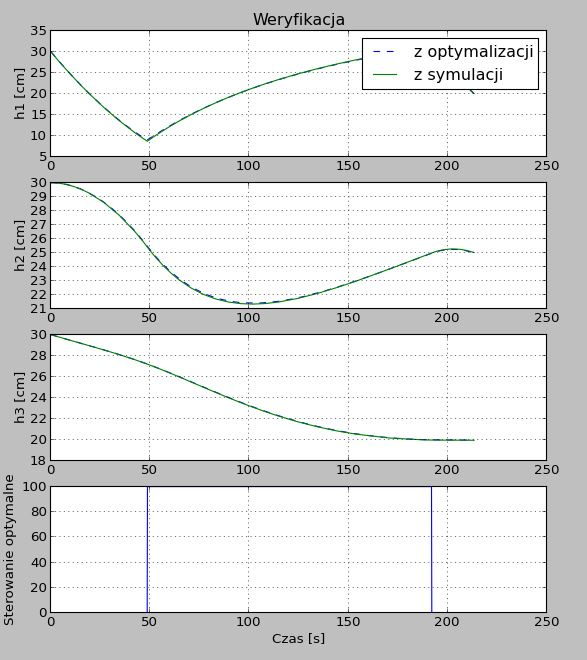
\includegraphics{Grafika/plot_30_30_30-20_25_20_normalised_200}
    \caption{Druga przykładowa weryfikacja po normalizacji sterowania. Źródło: własne.}
    \label{fig:plot303030-202520normalised200}
\end{figure}

Drugi przykład to upuszczanie niewielkiej ilości wody ze zbiorników od poziomów $h_{1}^{0} = 30 cm, h_{2}^{0} = 30 cm, h_{3}^{0} = 30 cm$ do $h_{1}^{f} = 20 cm, h_{2}^{f} = 25 cm, h_{3}^{f} = 20 cm$. Sterowanie w postaci ,,surowej'' osiągnęło wartość błędu weryfikacji $e_{wer}^{s} = 0,007$, a w postaci znormalizowanej: $e_{wer}^{n} = 0.019$. Tutaj różnica między błędami jest mniejsza niż w poprzednim przypadku, mimo bardziej skomplikowanej struktury sterowania wyznaczonego przez algorytm optymalizacyjny (pokazanego na rys. \ref{fig:plot303030-202520raw200}). Sterowanie znormalizowane zaprezentowano na rys. \ref{fig:plot303030-202520normalised200}. W tej optymalizacji użyto 200 elementów skończonych, więc trzeba to wziąć pod uwagę, porównując wartości błędów między oboma opisanymi przypadkami.


\subsubsection{Wpływ liczby elementów metody elementów skończonych na rozwiązanie}
%TODO: opisać wpływ liczby elementów na rozwiązanie

\begin{figure}[ht]
    \centering
    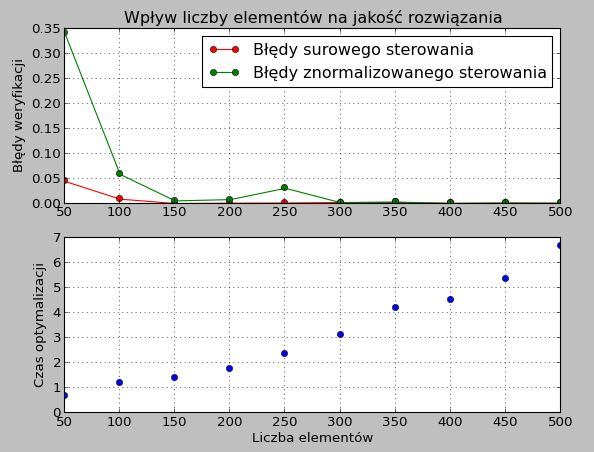
\includegraphics{Grafika/elements_influence_1-15_50-500}
    \caption{Wpływ liczby elementów skończonych na rozwiązanie. Źródło: własne.}
    \label{fig:elementsinfluence1-15_50-500}
\end{figure}

\begin{figure}[ht]
    \centering
    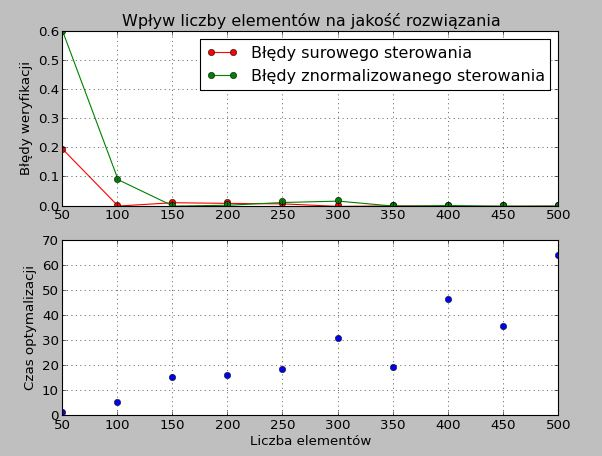
\includegraphics{Grafika/elements_influence_10-20_50-500}
    \caption{Drugi przykład wpływu liczby elementów skończonych na rozwiązanie. Źródło: własne.}
    \label{fig:elementsinfluence10-2050-500}
\end{figure}


%-------------------------------------------------
\subsection{Przy użyciu oprogramowania MATLAB/Simulink}
\label{sub:sym-wer-matlab}

%TODO: opisać okres próbkowania i inne ustawienia symulacji
%TODO: opisać wykresy i porównać z JModelicą

\begin{figure}
    \centering
    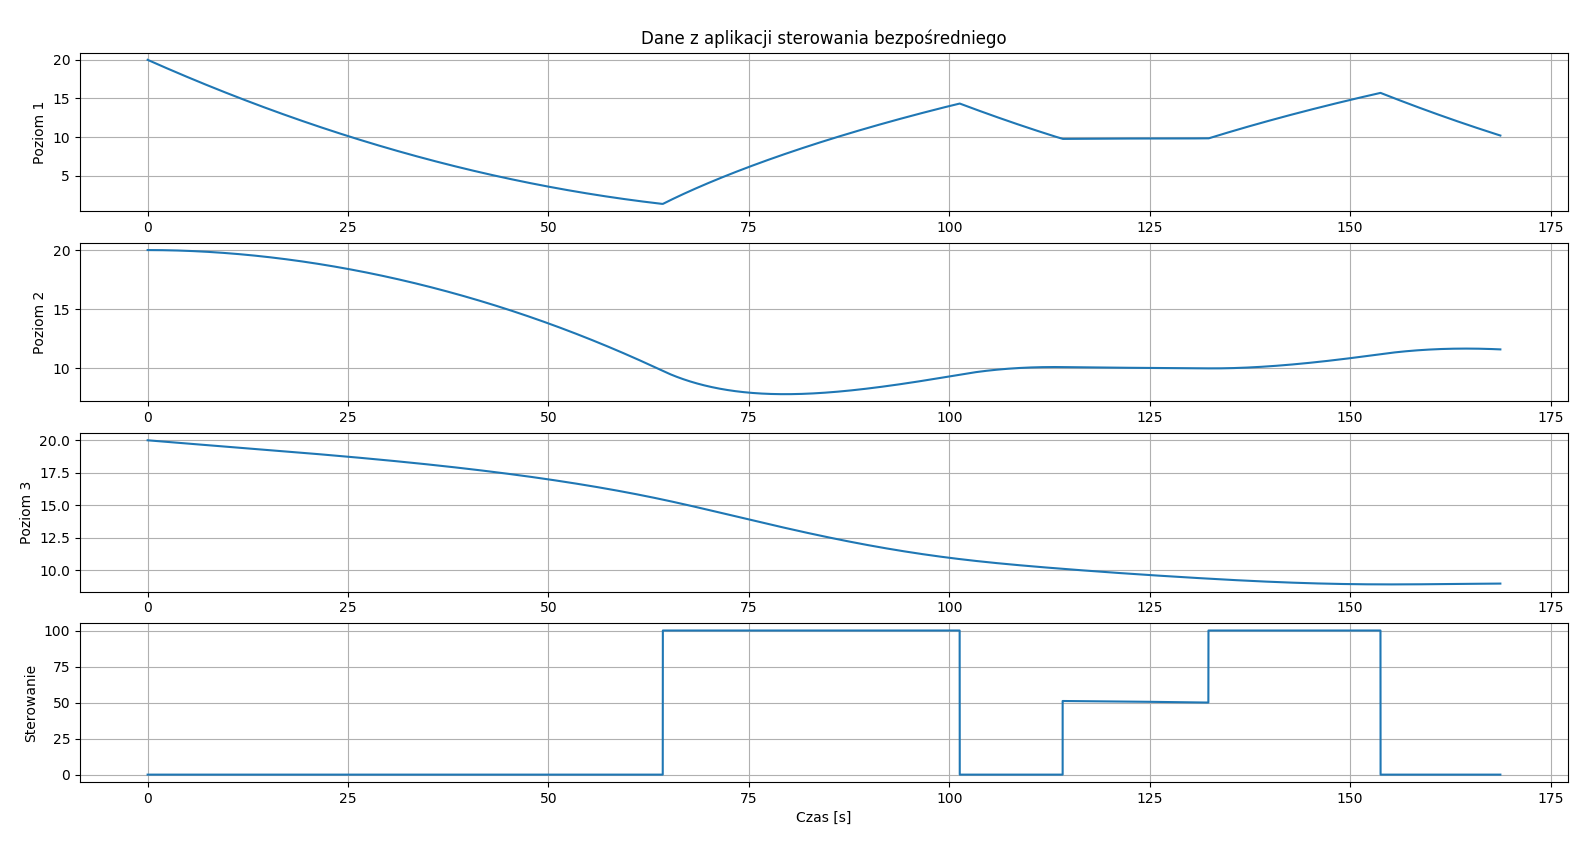
\includegraphics[scale=0.5,angle=90]{Grafika/ext_ctrl_2_opts}
    \caption{Dwa procesy optymalizacji zweryfikowane w symulacji niższym poziomem aplikacji. Źródło: własne.}
    \label{fig:extctrl2opts}
\end{figure}

\begin{figure}
    \centering
    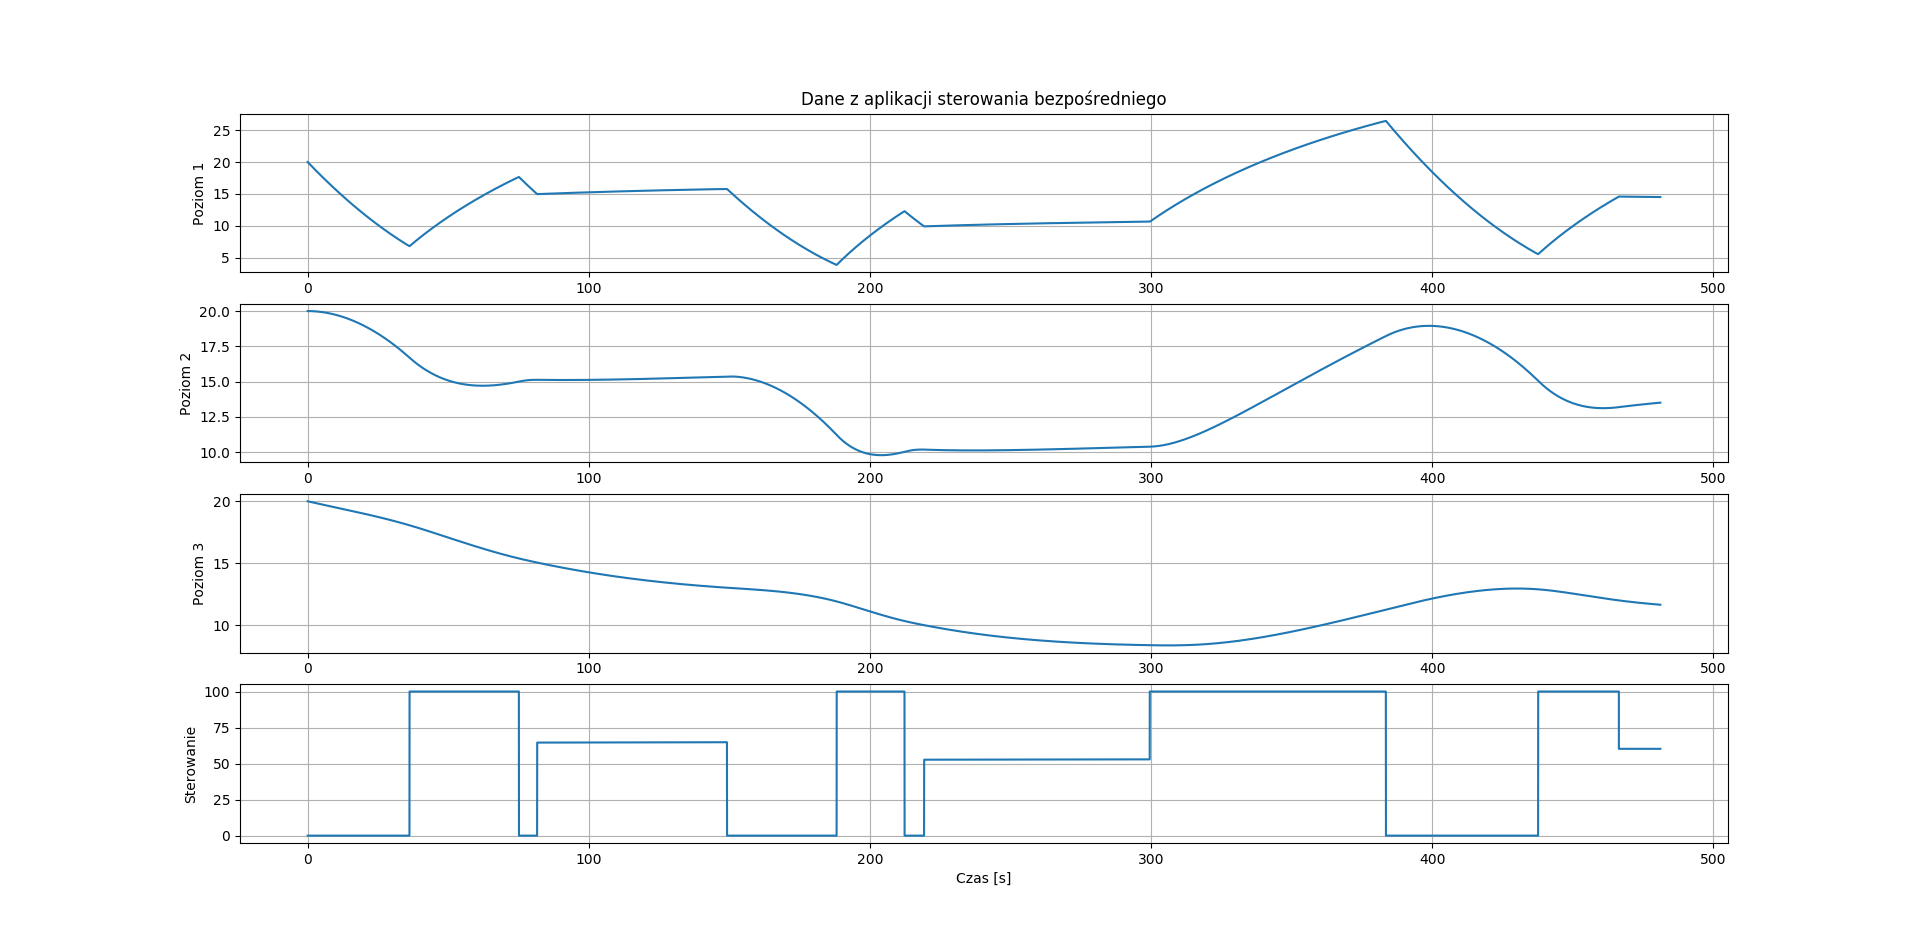
\includegraphics[scale=0.5,angle=90]{Grafika/ext_ctrl_3_opts}
    \caption{Trzy procesy optymalizacji zweryfikowane w symulacji niższego poziomu aplikacji. Źródło: własne.}
    \label{fig:extctrl3opts}
\end{figure}

%-------------------------------------------------
\subsection{Napotkane problemy}
\label{sub:sym-problems}

\subsubsection{Problemy z weryfikacją}

W przypadku niektórych wartości początkowych i końcowych oraz znalezionego dla nich sterowania optymalnego napotykano problem związany z tym, iż pakiet JModelica.org nie był w stanie obliczyć pochodnej jednego ze stanów w losowym punkcie czasu. Rozwiązano go poprzez zwiększenie liczby elementów skończonych przy rozwiązywaniu danego zadania. Nie zaobserwowano takich problemów przy liczbie elementów powyżej 50.

\subsubsection{Problem dostępności interfejsu systemu Tango}

Biblioteka Tango Controls nakłada jeszcze jedno ograniczenie na część obliczeniową aplikacji: interfejs powinien być dostępny z maksymalnie trzysekundowym opóźnieniem. To znaczy, że każda prośba klienta musi zostać obsłużona w ciągu 3 sekund. W przypadku operacji symulacji, a szczególnie optymalizacji to założenie nie jest spełnione, ponieważ szczególnie ta druga operacja może trwać nawet kilka minut.

W API Tango Controls do języka Python (nazywającym się PyTango) istnieją sposoby na asynchroniczne wywoływanie operacji (tzw. \emph{green modes}), ale mają dwie wady:
\begin{itemize}
    \item używają tylko jednego wątku głównego aplikacji,
    \item procedury pakietu JModelica.org są z nimi niekompatybilne.
\end{itemize}

W związku z tym zaproponowano własne, ogólne rozwiązanie problemu potrzeby asynchronicznego wykonywania operacji wewnątrz klasy urządzeń. W tym celu użyto biblioteki \texttt{multiprocessing} wchodzącej w skład standardowego zestawu narzędzi języka Python. Za jej pomocą zaimplementowano asynchroniczne wywoływanie długich operacji w osobnych procesach, które po swoim końcu wywołuja metody odwołania (ang. \emph{callback}) w głównym wątku aplikacji. Dzięki temu wszystkie komendy, które wywołują długie operacje (\emph{Optimise}, \emph{RunSimulation} oraz \emph{RunVerification}) tylko uruchamiają osobny proces i przypisują odpowiednią metodę odwołania, nie blokując interfejsu urządzenia.

Osobnym procesem jest również serwer TCP. Posiada on własny system logowania i komunikuje się z głównym procesem aplikacji wyższego poziomu poprzez potok danych (ang. \emph{pipe}, nie mylić z częścią interfejsu urządzenia systemu Tango). Jest on dwukierunkowy: serwer może przez niego wysyłać aktualne dane odebrane od aplikacji niższego poziomu, a główny proces wszystkie informacje o sterowaniu. Odbiór danych po stronie serwera znajduje się na początku pętli obsługi komunikacji z klientem TCP (aplikacją niższego poziomu). Odbiór danych po stronie urządzenia odbywa się w odpytywanej co 50 milisekund komendzie \emph{GetDataFromDirectControl}.

Użyto w tym celu procesów, a nie wątków ze względu na tzw. \emph{Global Interpreter Lock} - globalny zamek interpretera. Jest to cecha języka Python, która powoduje, że wątki nie mogą być uruchamiane równolegle (nawet w przypadku dostępnych rdzeni procesora), a zawsze są tylko współbieżne. Z kolei procesy nie są objęte tym ograniczeniem i można ich używać w prawdziwie równoległy sposób.
